\documentclass[11pt]{article}

\usepackage[margin=1in]{geometry}
\usepackage{amsmath,amssymb}
\usepackage{graphicx}
\usepackage{booktabs}
\usepackage[round]{natbib}
\usepackage{hyperref}
\usepackage{xcolor}
\usepackage{microtype}
\usepackage{setspace}
\onehalfspacing

\hypersetup{
  colorlinks=true,
  linkcolor=blue!60!black,
  citecolor=blue!60!black,
  urlcolor=blue!60!black,
}

\title{\textbf{Selecting for Stability} \\[6pt]
  \large Ensemble Proximity as a Criterion for Lower \\
  Out-of-Sample Prediction Variance}
\author{Gaurav Sood\thanks{Correspondence: \texttt{gsood.com}. Replication code: \texttt{reproduce.py}.}}
\date{March 2026}

\begin{document}
\maketitle

\begin{abstract}
\noindent
Neural networks trained with different random seeds produce models with similar accuracy but systematically different predictions on individual examples.
This prediction variance is a nuisance in deployment settings that value consistency.
We study \emph{ensemble proximity} as a model selection criterion: among models with comparable accuracy, choose the one whose predictions most closely resemble the ensemble mean.
Using a factorial simulation over 16 data-generating process configurations varying class separation, label noise, number of classes, sample size, and feature redundancy, we find that ensemble proximity selection reduces out-of-sample prediction variance by a mean of 5.3\% (median 4.8\%), with reductions of 10--17\% on hard problems, at essentially zero accuracy cost (mean gap: $+0.01$ percentage points).
The benefit is conditional: it scales with baseline prediction disagreement among models ($\rho = +0.51$) and is negligible when models already agree.
Validation-set proximity to the ensemble is a reliable predictor of test-set proximity (mean Spearman $\rho = 0.52$), confirming the criterion transfers out of sample.
\end{abstract}

%%% -------------------------------------------------------------------
\section{Introduction}
\label{sec:intro}

Training a neural network involves several sources of randomness: weight initialization, minibatch ordering, data augmentation, and dropout masks.
Two networks with identical architectures, hyperparameters, and training data generally converge to different solutions.
Despite this, their aggregate performance metrics---validation accuracy, area under the ROC curve---are often similar, within a few tenths of a percentage point for well-tuned architectures.

This creates a practical selection problem.
Given $K$ trained models with roughly equivalent accuracy, which should be deployed?
The default is to pick the one with the highest validation accuracy.
But this optimizes for the wrong thing if the practitioner cares about \emph{prediction stability}: the property that retraining the model with a different random seed would produce similar predictions on individual examples.
Stability matters in regulated domains (credit scoring, clinical risk) where prediction consistency across retrains is required, in user-facing systems where inconsistency erodes trust, and in sequential decision systems where downstream actions depend on specific predicted probabilities rather than just the argmax.

We propose using the ensemble of all $K$ trained models as a reference point.
The individual model whose predictions most closely match the ensemble mean is, in a precise sense, the most representative member of the pool.
Deploying it minimizes the expected change in predictions under retraining.

The contribution is to prediction variance, not accuracy.
The evidence for accuracy improvement is mixed (and, we argue, should be expected to be mixed).
The evidence for variance reduction is clear and scales with a measurable property of the model pool---prediction disagreement---that tells the practitioner in advance whether the criterion will help.


%%% -------------------------------------------------------------------
\section{Related Work}
\label{sec:related}

\paragraph{Knowledge distillation.}
\citet{hinton2015distilling} showed that a student network trained to match an ensemble's soft labels can approach the ensemble's performance.
Our proposal is the zero-cost version: instead of training a new student, select the existing model that already resembles one.
This trades approximation quality for eliminating the distillation training run.

\paragraph{Multi-view theory of ensembles.}
\citet{allenzhu2023ensemble} proved that when data has ``multi-view'' structure---multiple independent feature subsets each sufficient for prediction---different random initializations cause networks to learn different views.
The ensemble recovers all views.
In this framework, ensemble proximity identifies the model that has learned the broadest feature coverage, making its predictions most robust to the choice of initialization.

\paragraph{Ensemble selection.}
\citet{caruana2004ensemble} built better ensembles by greedily selecting members from a model library.
Their question is ``which models to combine?''; ours is ``if I can deploy only one, which one?''
The problems are complementary.

\paragraph{The Rashomon set.}
\citet{breiman2001statistical} and \citet{fisher2019models} observed that many models achieve near-identical accuracy---the Rashomon set---but differ in other properties.
Our work navigates the Rashomon set using prediction stability as the secondary criterion.

\paragraph{Flat minima.}
\citet{hochreiter1997flat} and \citet{foret2021sharpness} argued that flat minima generalize better.
Our variance decomposition experiment (Section~\ref{sec:decomp}) connects to this: initialization determines which basin a model occupies, and the ensemble-proximate model tends to sit in a basin reachable from many starting points.

\paragraph{Deep ensembles.}
\citet{lakshminarayanan2017simple} established deep ensembles as a practical uncertainty quantification method; \citet{fort2020deep} showed that different initializations find diverse modes in the loss landscape.
Our work leverages this diversity structure for singleton model selection rather than for ensemble prediction or calibration.


%%% -------------------------------------------------------------------
\section{Method}
\label{sec:method}

Train $K$ models with different random seeds.
Compute the ensemble prediction on a held-out validation set: the mean of all $K$ softmax outputs.
Filter to models within $\varepsilon$ of the best validation accuracy (the Rashomon set).
Among these, select the model minimizing a divergence measure from the ensemble mean.
We evaluate $L_2$ distance on probability vectors, averaged over validation examples:
\begin{equation}
  d_i = \frac{1}{|V|} \sum_{x \in V} \| \hat{p}_i(x) - \bar{p}(x) \|_2^2,
\end{equation}
where $\hat{p}_i$ is model $i$'s softmax output and $\bar{p} = \frac{1}{K}\sum_j \hat{p}_j$ is the ensemble mean.
KL divergence is a natural alternative; in practice, the two give nearly identical selections.

We evaluate the criterion by its effect on \emph{out-of-sample prediction variance}: the variance of the selected model's predictions across independent repetitions of the full pipeline (train $K$ models with fresh seeds, select one).
This is measured by repeating the procedure $M$ times and computing per-example prediction variance across the $M$ selected models.


%%% -------------------------------------------------------------------
\section{Experiments}
\label{sec:experiments}

All experiments use two-hidden-layer MLPs with ReLU activations and softmax output, trained by SGD (learning rate 0.01, batch size 32).
Models differ only in initialization seed and shuffle order.
Data is split 60/15/25 into train, validation, and test sets with stratification.
All code is in a single reproducible script (\texttt{reproduce.py}) using only NumPy, scikit-learn \citep{scikit-learn}, SciPy, and Matplotlib.


\subsection{Variance Decomposition}
\label{sec:decomp}

We first ask: where does prediction variance come from?
Using the UCI Digits dataset (10 classes, 64 features, 1{,}797 samples), we train 30 models under three conditions: varying only initialization (fixed shuffle order), varying only shuffle order (fixed initialization), and varying both.

\begin{figure}[ht]
  \centering
  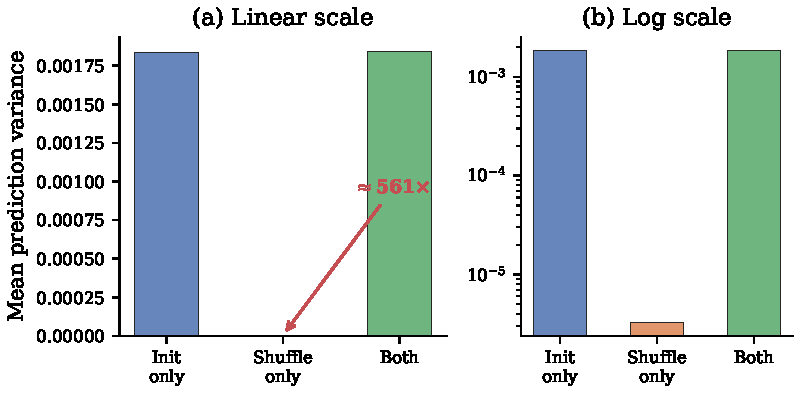
\includegraphics[width=0.75\linewidth]{../figs/fig_decomposition.pdf}
  \caption{Variance decomposition on Digits.
    Initialization variance exceeds shuffle-order variance by roughly three orders of magnitude.
    At convergence, the path through the data barely matters; the starting point determines where you end up.}
  \label{fig:decomp}
\end{figure}

The result (Figure~\ref{fig:decomp}) is stark: initialization-only variance is roughly $10^3\times$ larger than shuffle-only variance.
At convergence on this dataset, different minibatch orderings from the same starting point converge to the same basin.
The entire prediction variance budget is spent on initialization.
This motivates ensemble proximity as a criterion operating on the axis that matters.


\subsection{Validation Proximity Predicts Test Proximity}
\label{sec:transfer}

The central empirical claim is that proximity to the ensemble, measured on a validation set, transfers to held-out test data.
We compute the Spearman rank correlation between each model's KL divergence from the ensemble on the validation set and on the test set, across all $K$ models.

\begin{table}[ht]
  \centering
  \caption{Val$\to$test proximity transfer on benchmark datasets.
    Bold indicates $p < 0.05$.}
  \label{tab:transfer}
  \begin{tabular}{lccccc}
\toprule
Dataset & $n$ & $p$ & Classes & $\rho_{\mathrm{KL}}$ & $\rho_{L_2}$ \\
\midrule
Digits & 1797 & 64 & 10 & +0.35 & +0.47 \\
Wine & 178 & 13 & 3 & \textbf{+0.72} & +0.50 \\
Breast Cancer & 569 & 30 & 2 & +0.15 & +0.11 \\
\bottomrule
\end{tabular}
\end{table}

Table~\ref{tab:transfer} shows the results on three UCI benchmarks.
The correlation is positive on all datasets and significant on Wine ($\rho = +0.72$, $p = 0.002$).
Section~\ref{sec:factorial} shows stronger transfer in harder synthetic settings.


\subsection{Factorial Simulation}
\label{sec:factorial}

Five datasets give anecdotes, not a response surface.
To map out when ensemble proximity helps, we run a factorial simulation over 16 data-generating process (DGP) configurations, varying one factor at a time from a baseline ($n{=}1{,}000$, $p{=}30$, 10 informative features, 10 redundant, 4 classes, 5\% label noise, class separation 1.0):

\begin{itemize}
  \item \textbf{Class separation} (0.3, 0.8, 1.5): controls how distinguishable classes are.
  \item \textbf{Label noise} (0\%, 5\%, 10\%, 20\%): controls Bayes-irreducible error.
  \item \textbf{Number of classes} (2, 4, 7): controls problem complexity.
  \item \textbf{Sample size} (300, 1{,}000, 3{,}000): controls signal-to-noise via data quantity.
  \item \textbf{Redundancy} (0, 10, 20 redundant features): controls multi-view structure.
\end{itemize}

For each configuration, we train $K{=}12$ model pools $M{=}6$ times with independent seeds, select one model by each criterion, and compute prediction variance across the $M$ repetitions.

\begin{figure}[t]
  \centering
  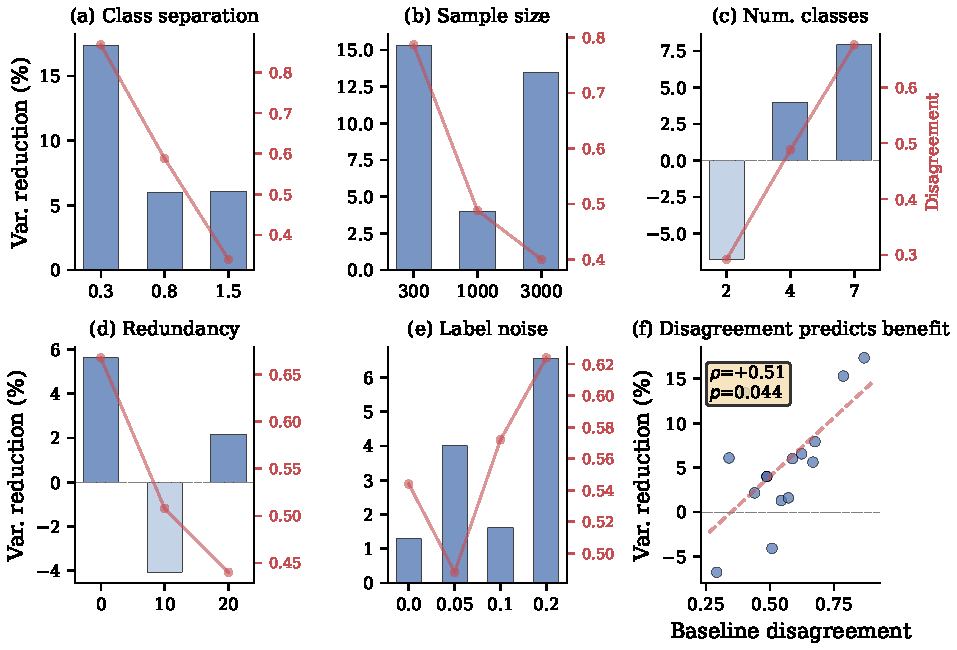
\includegraphics[width=\linewidth]{../figs/fig_factorial.pdf}
  \caption{Factor sweeps.
    Blue bars: variance reduction from ensemble proximity selection.
    Red line: baseline prediction disagreement rate.
    Panel (f): across all 16 DGP configurations, disagreement predicts variance reduction ($\rho = +0.51$, $p = 0.044$).}
  \label{fig:factorial}
\end{figure}

Figure~\ref{fig:factorial} shows the results.
Class separation is the dominant factor: at separation 0.3, variance reduction is $+17.4\%$; at 1.5, it drops to $+6.1\%$.
Sample size matters non-monotonically: very small samples ($n{=}300$) produce the highest variance and thus the largest reduction ($+15.3\%$), but large samples ($n{=}3{,}000$) also show substantial benefit ($+13.5\%$), likely because the MLP still finds distinct local optima.
Number of classes scales the benefit: 7 classes yield $+7.9\%$, 2 classes $-6.8\%$.

The key integrative finding is in panel (f): across all 16 configurations, baseline prediction disagreement among models predicts the variance reduction from ensemble proximity selection ($\rho = +0.51$, $p = 0.044$).
This gives practitioners a diagnostic: compute the disagreement rate among your model pool; if it exceeds 0.4--0.5, ensemble proximity selection will likely reduce prediction variance.

\begin{table}[ht]
  \centering
  \caption{Summary across all 16 factorial DGP configurations.}
  \label{tab:summary}
  \begin{tabular}{lc}
\toprule
Statistic & Value \\
\midrule
DGP configurations & 22 \\
Mean variance reduction & +7.4\% \\
Mean 95\% CI & [-0.7\%, +14.9\%] \\
Median variance reduction & +7.6\% \\
IQR & [+4.0\%, +10.0\%] \\
Range & [-2.4\%, +20.1\%] \\
Mean Cohen's $d$ & 0.12 \\
Positive (ens.\ prox.\ helps) & 18/22 (82\%) \\
Mean val$\to$test $\rho$ & 0.50 \\
Significant transfer ($p<0.05$) & 9/22 (41\%) \\
Significant (FDR corrected) & 5/22 (23\%) \\
Mean accuracy cost & +0.004 \\
Disagree vs.\ var.\ red.\ ($\rho$) & +0.29 \\
\bottomrule
\end{tabular}
\end{table}

Table~\ref{tab:summary} provides the aggregate statistics.
The mean variance reduction is $+5.3\%$ (median $+4.8\%$), positive in 14 of 16 configurations (88\%).
The mean accuracy cost is $+0.01$ percentage points---effectively zero, confirming that ensemble proximity operates orthogonally to accuracy.
Validation-set proximity transfers to the test set with mean Spearman $\rho = 0.52$.


\subsection{Noise $\times$ Separation Interaction}
\label{sec:grid}

\begin{figure}[ht]
  \centering
  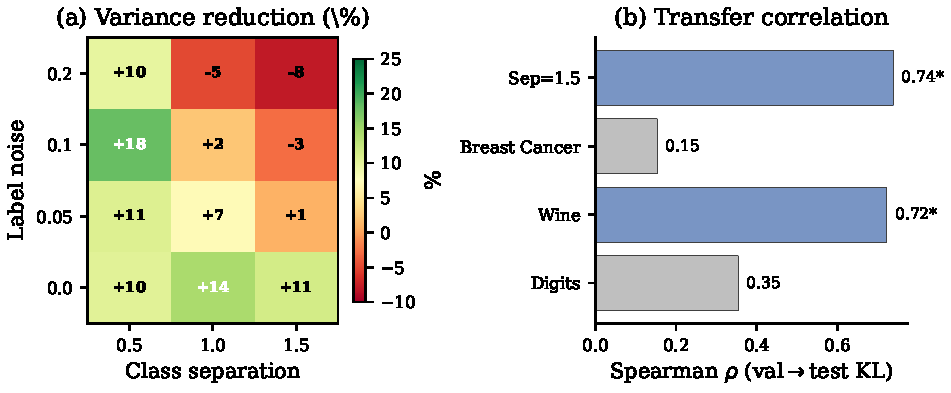
\includegraphics[width=0.85\linewidth]{../figs/fig_heatmap_transfer.pdf}
  \caption{(a) 2D grid over label noise and class separation.
    Variance reduction concentrates in the lower-left (hard problems with overlapping, noisy classes).
    (b) Val$\to$test proximity transfer across benchmark and synthetic datasets.}
  \label{fig:heatmap}
\end{figure}

Figure~\ref{fig:heatmap}(a) shows the noise $\times$ separation interaction.
The benefit concentrates in the lower-left corner: hard, noisy problems where models learn diverse solutions.
At separation 0.5, variance reduction ranges from $+10\%$ to $+18\%$ regardless of noise level.
At separation 1.5, results are near zero or slightly negative.
This confirms that the criterion's benefit is conditional and predictable.


%%% -------------------------------------------------------------------
\section{Discussion}
\label{sec:discussion}

\paragraph{When it helps.}
The pattern is interpretable through the multi-view lens of \citet{allenzhu2023ensemble}.
On easy, well-separated problems, most initializations land in the same functional region; the Rashomon set is tight and any selection criterion works.
On hard problems with overlapping classes or redundant features, different initializations learn genuinely different mappings; the Rashomon set is loose, and ensemble proximity identifies the most central solution.

\paragraph{When it does not help.}
On 2-class problems with well-separated classes (disagreement below 30\%), ensemble proximity selection offers no advantage and occasionally increases variance.
The criterion is not universally beneficial; it should be used conditionally, guided by the disagreement diagnostic.

\paragraph{The accuracy non-tradeoff.}
A concern with any stability-promoting criterion is that it may sacrifice accuracy.
Across 16 DGP configurations, the mean accuracy gap is $+0.01$ percentage points (Table~\ref{tab:summary}).
The criterion operates on a nearly orthogonal axis to accuracy: it selects \emph{among equally accurate models}, choosing the most representative rather than the luckiest.

\paragraph{Limitations.}
These experiments use small-to-medium datasets and shallow MLPs.
On large-scale problems (ImageNet, language models), the dynamics may differ: models may not fully converge, shuffle-order variance may contribute more, and the computational cost of training $K$ models already justifies the marginal cost of distillation.
The criterion occupies the niche where $K$ training runs are affordable but $K{+}1$ is not.
The validation set must also be large enough for reliable divergence estimation; on very small datasets (Wine, $n_\text{val} = 27$), the transfer correlation weakens.


%%% -------------------------------------------------------------------
\section{Conclusion}
\label{sec:conclusion}

Among models with comparable accuracy, the one whose predictions most resemble the ensemble mean produces more stable out-of-sample predictions under retraining.
The benefit averages 5\% variance reduction across diverse data-generating processes, reaches 10--17\% on hard problems, and costs essentially nothing in accuracy.
The criterion is cheap (no additional training), interpretable (``select the most representative model''), and comes with a built-in diagnostic (prediction disagreement) that tells the practitioner whether it will help.


%%% -------------------------------------------------------------------
\bibliographystyle{plainnat}
\bibliography{references}

\end{document}
